% TODO CTRL+F: TODO, ???,  SMAZAT, <expand>
% TODO poradne si procti projekt.pdf z navod/ Appendix A, jsou tam body co musis udelat


%==============================================================================
% tento soubor pouzijte jako zaklad
% this file should be used as a base for the thesis
% (c) 2008 Michal Bidlo
% E-mail: bidlom AT fit vutbr cz
% Šablonu upravil / template edited by: Ing. Jaroslav Dytrych, dytrych@fit.vutbr.cz
%==============================================================================
% kodovaní: UTF-8 (zmena prikazem iconv, recode nebo cstocs)
% encoding: UTF-8 (you can change it by command iconv, recode or cstocs)
%------------------------------------------------------------------------------
% zpracování / processing: make, make pdf, make clean
%==============================================================================
% Soubory, které je nutné upravit: / Files which have to be edited:
%   projekt-20-literatura-bibliography.bib - literatura / bibliography
%   projekt-01-kapitoly-chapters.tex - obsah práce / the thesis content
%   projekt-30-prilohy-appendices.tex - přílohy / appendices
%==============================================================================
%\documentclass[czech]{fitthesis} % bez zadání - pro začátek práce, aby nebyl problém s překladem
\documentclass[english]{fitthesis} % without assignment - for the work start to avoid compilation problem
%\documentclass[zadani]{fitthesis} % odevzdani do wisu - odkazy jsou barevné
%\documentclass[english,zadani]{fitthesis} % for submission to the IS FIT - links are color
%\documentclass[zadani,print]{fitthesis} % pro tisk - odkazy jsou černé
%\documentclass[english,zadani,print]{fitthesis} % for the print - links are black
% * Je-li prace psana v anglickem jazyce, je zapotrebi u tridy pouzit 
%   parametr english nasledovne:
%   If thesis is written in english, it is necessary to use 
%   parameter english as follows:
%      \documentclass[english]{fitthesis}
% * Je-li prace psana ve slovenskem jazyce, je zapotrebi u tridy pouzit 
%   parametr slovak nasledovne:
%      \documentclass[slovak]{fitthesis}

% Základní balíčky jsou dole v souboru šablony fitthesis.cls
% Basic packages are at the bottom of template file fitthesis.cls
%zde muzeme vlozit vlastni balicky / you can place own packages here

\usepackage{graphicx}
\graphicspath{ {obrazky-figures/} }

%---rm---------------
\renewcommand{\rmdefault}{lmr}%zavede Latin Modern Roman jako rm / set Latin Modern Roman as rm
%---sf---------------
\renewcommand{\sfdefault}{qhv}%zavede TeX Gyre Heros jako sf
%---tt------------
\renewcommand{\ttdefault}{lmtt}% zavede Latin Modern tt jako tt

% vypne funkci šablony, která automaticky nahrazuje uvozovky,
% aby nebyly prováděny nevhodné náhrady v popisech API apod.
% disables function of the template which replaces quotation marks
% to avoid unnecessary replacements in the API descriptions etc.
\csdoublequotesoff

% =======================================================================
% balíček "hyperref" vytváří klikací odkazy v pdf, pokud tedy použijeme pdflatex
% problém je, že balíček hyperref musí být uveden jako poslední, takže nemůže
% být v šabloně
% "hyperref" package create clickable links in pdf if you are using pdflatex.
% Problem is that this package have to be introduced as the last one so it 
% can not be placed in the template file.
\ifWis
\ifx\pdfoutput\undefined % nejedeme pod pdflatexem / we are not using pdflatex
\else
  \usepackage{color}
  \usepackage[unicode,colorlinks,hyperindex,plainpages=false,pdftex]{hyperref}
  \definecolor{links}{rgb}{0.4,0.5,0}
  \definecolor{anchors}{rgb}{1,0,0}
  \def\AnchorColor{anchors}
  \def\LinkColor{links}
  \def\pdfBorderAttrs{/Border [0 0 0] }  % bez okrajů kolem odkazů / without margins around links
  \pdfcompresslevel=9
\fi
\else % pro tisk budou odkazy, na které se dá klikat, černé / for the print clickable links will be black
\ifx\pdfoutput\undefined % nejedeme pod pdflatexem / we are not using pdflatex
\else
  \usepackage{color}
  \usepackage[unicode,colorlinks,hyperindex,plainpages=false,pdftex,urlcolor=black,linkcolor=black,citecolor=black]{hyperref}
  \definecolor{links}{rgb}{0,0,0}
  \definecolor{anchors}{rgb}{0,0,0}
  \def\AnchorColor{anchors}
  \def\LinkColor{links}
  \def\pdfBorderAttrs{/Border [0 0 0] } % bez okrajů kolem odkazů / without margins around links
  \pdfcompresslevel=9
\fi
\fi
% Řešení problému, kdy klikací odkazy na obrázky vedou za obrázek
% This solves the problems with links which leads after the picture
\usepackage[all]{hypcap}

% Informace o práci/projektu / Information about the thesis
%---------------------------------------------------------------------------
\projectinfo{
  %Prace / Thesis
  project=BP,            %typ prace BP/SP/DP/DR  / thesis type (SP = term project)
  year=2017,             %rok odevzdání / year of submission
  date=\today,           %datum odevzdani / submission date
  %Nazev prace / thesis title
  title.cs={Optimalizace výkonu automatizované testovací platformy založené na Beakerlibu},  %nazev prace v cestine ci slovenstine (dle zadani) / thesis title in czech language (according to assignment)
  title.en={Performance Optimization of Testing  Automation Framework Based on Beakerlib}, %nazev prace v anglictine / thesis title in english
  %Autor / Author
  author={Jakub Heger},   %cele jmeno a prijmeni autora / full name and surname of the author
  author.name={Jakub},   %jmeno autora (pro citaci) / author name (for reference) 
  author.surname={Heger},   %prijmeni autora (pro citaci) / author surname (for reference) 
  %author.title.p=Bc., %titul pred jmenem (nepovinne) / title before the name (optional)
  %author.title.a=PhD, %titul za jmenem (nepovinne) / title after the name (optional)
  %Ustav / Department
  department=DITS, % doplnte prislusnou zkratku dle ustavu na zadani: UPSY/UIFS/UITS/UPGM
  %                  fill in appropriate abbreviation of the department according to assignment: UPSY/UIFS/UITS/UPGM
  %Skolitel / supervisor
  supervisor={Hana Pluháčková}, %cele jmeno a prijmeni skolitele / full name and surname of the supervisor
  supervisor.name={Hana},   %jmeno skolitele (pro citaci) / supervisor name (for reference) 
  supervisor.surname={Pluháčková},   %prijmeni skolitele (pro citaci) / supervisor surname (for reference) 
  supervisor.title.p={Mgr. Bc.},   %titul pred jmenem (nepovinne) / title before the name (optional)
%  supervisor.title.a={},    %titul za jmenem (nepovinne) / title after the name (optional)
  %Klicova slova, abstrakty, prohlaseni a podekovani je mozne definovat 
  %bud pomoci nasledujicich parametru nebo pomoci vyhrazenych maker (viz dale)
  %Keywords, abstracts, declaration and acknowledgement can be defined by following 
  %parameters or using dedicated macros (see below)
  %===========================================================================
  %Klicova slova / keywords
  %keywords.cs={Klíčová slova v českém jazyce.}, %klicova slova v ceskem ci slovenskem jazyce
  %                                              keywords in czech or slovak language
  %keywords.en={Klíčová slova v anglickém jazyce.}, %klicova slova v anglickem jazyce / keywords in english
  %Abstract
  %abstract.cs={Výtah (abstrakt) práce v českém jazyce.}, % abstrakt v ceskem ci slovenskem jazyce
  %                                                         abstract in czech or slovak language
  %abstract.en={Výtah (abstrakt) práce v anglickém jazyce.}, % abstrakt v anglickem jazyce / abstract in english
  %Prohlaseni / Declaration
  %declaration={Prohlašuji, že jsem tuto bakalářskou práci vypracoval samostatně pod vedením pana ...},
  %Podekovani (nepovinne) / Acknowledgement (optional)
  %acknowledgment={Zde je možné uvést poděkování vedoucímu práce a těm, kteří poskytli odbornou pomoc.} % nepovinne
  %acknowledgment={Here it is possible to express thanks to the supervisor and to the people which provided professional help.} % optional
}

%Abstrakt (cesky, slovensky ci anglicky) / Abstract (in czech, slovak or english)
\abstract[cs]{Do tohoto odstavce bude zapsán výtah (abstrakt) práce v českém (slovenském) jazyce.}
\abstract[en]{Do tohoto odstavce bude zapsán výtah (abstrakt) práce v anglickém jazyce.}

%Klicova slova (cesky, slovensky ci anglicky) / Keywords (in czech, slovak or english)
\keywords[cs]{Sem budou zapsána jednotlivá klíčová slova v českém (slovenském) jazyce, oddělená čárkami.}
\keywords[en]{Sem budou zapsána jednotlivá klíčová slova v anglickém jazyce, oddělená čárkami.}

%Prohlaseni (u anglicky psane prace anglicky, u slovensky psane prace slovensky)
%Declaration (for thesis in english should be in english)
\declaration{Prohlašuji, že jsem tuto bakalářskou práci vypracoval samostatně pod vedením paní Mgr. Bc. Hany Pluháčkové.
Další informace mi poskytl Mgr. David Kutálek. ???
Uvedl jsem všechny literární prameny a publikace, ze kterých jsem čerpal.}

% \declaration{Hereby I declare that this bachelor's thesis was prepared as an original author’s work under the supervision of Mr. X
% The supplementary information was provided by Mr. Y
% All the relevant information sources, which were used during preparation of this thesis, are properly cited and included in the list of references.}

%Podekovani (nepovinne, nejlepe v jazyce prace) / Acknowledgement (optional, ideally in the language of the thesis)
\acknowledgment{V této sekci je možno uvést poděkování vedoucímu práce a těm, kteří poskytli odbornou pomoc
(externí zadavatel, konzultant, apod.).}
%\acknowledgment{Here it is possible to express thanks to the supervisor and to the people which provided professional help
%(external submitter, consultant, etc.).}

% řeší první/poslední řádek odstavce na předchozí/následující stránce
% solves first/last row of the paragraph on the previous/next page
\clubpenalty=10000
\widowpenalty=10000

\begin{document}
  % Vysazeni titulnich stran / Typesetting of the title pages
  % ----------------------------------------------
  \maketitle
  % Obsah
  % ----------------------------------------------
  \tableofcontents
  
  % Seznam obrazku a tabulek (pokud prace obsahuje velke mnozstvi obrazku, tak se to hodi)
  % List of figures and list of tables (if the thesis contains a lot of pictures, it is good)
\ifczech
  \renewcommand\listfigurename{Seznam obrázků}
\fi
\ifslovak
  \renewcommand\listfigurename{Zoznam obrázkov}
\fi

  % \listoffigures
\ifczech
  \renewcommand\listtablename{Seznam tabulek}
\fi
\ifslovak
  \renewcommand\listtablename{Zoznam tabuliek}
\fi

  % \listoftables 

  % vynechani stranky v oboustrannem rezimu
  % Skip the page in the two-sided mode
  \iftwoside
    \cleardoublepage
  \fi

% Listing settings
\lstset{basicstyle=\ttfamily,
  morekeywords={rlRun, PACKAGE},
  showstringspaces=false,
  commentstyle=\color{red},
  keywordstyle=\color{blue},
  numbers=left,
  stepnumber=1,    
  firstnumber=1,
  numberfirstline=true,
  captionpos=b
}

\lstdefinestyle{beakerlib_bash}{
language=bash,
keywordstyle=\color{blue},
commentstyle=\color{gray},
stringstyle=\color{orange},
numbers=left,
stepnumber=1,
numbersep=5pt,
numberstyle=\tiny,
breaklines=true,
breakautoindent=true,
breakatwhitespace=false,
postbreak=\space,
tabsize=2,
basicstyle=\ttfamily\scriptsize,
showspaces=false,
showstringspaces=false,
extendedchars=true,
backgroundcolor=\color{white},
morekeywords={rlRun, rlPhaseStartTest, rlPhaseEnd, rlPhaseStartTest, rlPhaseStartCleanup, rlAssertRpm, rlJournalPrint, rlJournalEnd, rlJournalStart, rlAssertExists, rlPhaseStartSetup}
 }

\lstdefinestyle{txt}{
basicstyle=\tiny,
keywordstyle=\color{blue},
commentstyle=\color{gray},
stringstyle=\color{orange},
numbers=left,
stepnumber=1,
numbersep=5pt,
numberstyle=\tiny,
breaklines=true,
breakautoindent=true,
breakatwhitespace=false,
postbreak=\space,
tabsize=2,
basicstyle=\ttfamily\scriptsize,
showspaces=false,
showstringspaces=false,
extendedchars=true,
backgroundcolor=\color{white},
morekeywords={}
 }


  % Text prace / Thesis text
  % ----------------------------------------------
  %=========================================================================
% (c) Michal Bidlo, Bohuslav Křena, 2008

% Start of text
\chapter{Introduction}

Focus of this thesis is a performance optimization of Red Hat's BeakerLib library, particularly its Journal feature. <expand>
\\
\\
The thesis is structured in a following way: chapter \ref{relevant_projects} introduces projects relevant to BeakerLib and its testing environment. Chapter \ref{beakerlib_chapter} explains more in-depth how BeakerLib works, with focus on its Journal feature and analysis of its performance. 

In the chapter \ref{solutions} possible optimizations are discussed and chapter \ref{implementations} focuses on implementation of proposed solutions. The chapter \ref{performance} then describes how was performance measured and in what environment. Chapter \ref{results}  is dedicated to analyses of measured results. 

Lastly chapter \ref{conclusion} sums up implemented solutions a  considers possible future work on BeakerLib.

\chapter{Relevant projects}
\label{relevant_projects}

This this chapter describes BeakerLib and projects relevant to it. First of all brief summary of BeakerLib itself is presented. Next section is devoted to Beaker system and last section  Nejprve je popsana knihovna jako takova, nasledujici sekce se venuje Beaker coz je system from which BeakrLib originally  a posledni sekce popisuje test harnessy

\section{BeakerLib}

BeakerLib is a Linux shell-level integration testing library, providing convenience functions which simplify writing, running and analysis of integration and blackbox tests. \cite{beakerlib_wiki}
It is developed and maintained by Red Hat and operates under GNU General Public License.
Main features of BeakerLib include:
\begin{itemize}
\item Journal - uniform logging mechanism (logs and results saved in flexible XML format, easy to compare results and generate reports)
\item Phases - logical grouping of test actions, clear separation of setup / test / cleanup
\item Asserts - common checks affecting the overall results of individual phases (checking for exit codes, file existence and content...)
\item Helpers - convenience functions for common operations such as managing system services, backup and restore of files and more
\end{itemize}


This thesis focuses on BeakerLib Journal feature and problem it causes with long tests. Which is in more detail described in chapter \ref{beakerlib_chapter}.


\section{Beaker}

Beaker\cite{beaker_doc} is a full stack software and hardware integration testing system, with the ability to manage a globally distributed network of test labs.  It is Red Hat community project under GNU General Public License version 2.

Main functionality includes management of hardware inventory, on which Beaker can install wide variety  of operating systems from Red Hat Linux family. Another notable part  is Task library which contains rpm packages of individual tests which can be run on provided machines. 
Users then can specify which hardware they require with which OS and tests they want to run on it through either command-line tools or web interface both of which are part of Beaker install package. If Beaker meets given criteria in its inventory it installs Test harness to which it gives list of tests to be run.  Test Harness install and executes them while continuously sending results back to Beaker where they are stored for specified period of time. 

\subsection{beaker-wizard}
Part of Beaker package. Interactive command-line tool which automates creation of BeakerLib tests. Using predefined or user-defined templates it creates all files that are needed to run BeakerLib test. 
???  Common use cases

\section{Test Harness}
Test harness is a software framework that automates test execution. It contains tests to be run, executes them and reports results. <expand>

Beaker’s harnesses prepare provided machine for BeakerLib by setting environmental variables to proper values, and then consecutively execute each test, while continuously reporting back results. They are integral part of Beaker ecosystem, as they allow user to run long test sets, whcih would without harness require much of manual work.

\subsection{Beah harness}
Beah \cite{beah_doc} is a default Beaker harness . <expand> 

\subsection{Restraint harness}
Restraint \cite{restraint_doc} is an alternative Beaker harness which can, unlike Beah, run with Beaker or standalone without it. <expand>

\section{Projects' relation}
Relation between Beaker, Harness and BeakerLib is shown in figure \ref{fig:beaker_relation}. In this example user submits Beaker job containing three tests and hardware/software requirements for a machine the tests should run on. After Beaker reserves it, it installs operating system and Harness which then successively executes each test and uploads their results back to Beaker when user can access them.

\begin{figure}[h!]
  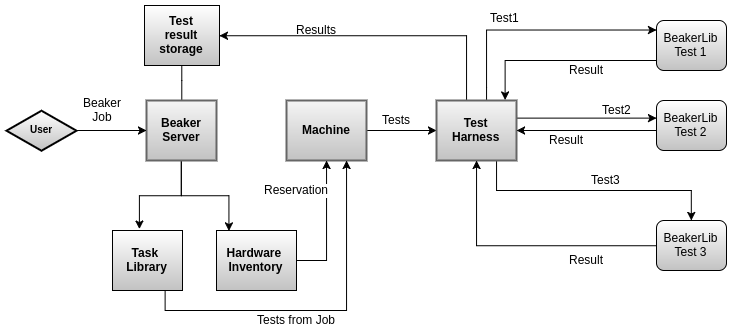
\includegraphics[width=\linewidth]{beaker_relations.png}
  \caption{Beaker relation to BeakerLib}
  \label{fig:beaker_relation}
\end{figure}

\chapter{BeakerLib}
\label{beakerlib_chapter}

This chapter takes a closer look on inner workings of BeakerLib, with focus on Journal feature and performance issues it suffers from. 

\section{Important functions}
As stated earlier BeakerLib is shell-level library with functions that make writing and running tests easier as well as examining their results.
BeakerLib adds testing functions to \texttt{shell} functionality, so user can combine normal \texttt{shell} commands and constructions with helping functions which can make writing tests and examining their results easier. There is close to 80 of these functions (also known as \textbf{rlCommands}), description of most used ones follows:
\begin{itemize}
\item \texttt{rlRun()} - First argument of this function is any \texttt{shell} command, which is executed by \texttt{rlRun()}. Second is an expected exit code of first argument, it can contain one or more codes. Third argument is a comment. BeakerLib logs \texttt{FAIL} or \texttt{PASS} if expected exit code differs or not from actual one respectively along with comment. This is most used and important function.
\item \texttt{rlPass()} - Manual assertion and logging of \texttt{PASS}. Useful when in combination with if statement which user doesn't want to appear in logs but still wants to log its result. Reciprocal function \texttt{rlFail()} exists as well.
\item \texttt{rlAssertExists} - Asserts whether file given as a first argument exists.
\item \texttt{rlAssertGrep()} - Function logs \texttt{PASS} when pattern given as first argument matches in a file which is given a second argument. Optional flags are passed to \texttt{grep} and behave the same way.
\item \texttt{rlAssertRpm()} - Function asserts \texttt{PASS} when package given as first argument is installed.  Optional arguments allow specifying particular version, release or arch of the package.
\item \texttt{rlAssertDiffer()} - Asserts whether two files given as argument differ in their content. 
\item \texttt{rlJournalStart()} - This function is used at the start of each test. It is essential for proper run of the test as it initializes BeakerLib's  outputs, which described later in this chapter. Reciprocal function \textbf{rlJournalEnd()} must be called at the end of the test.
\item \texttt{rlPhaseStart()} - This function starts user-defined phase. Function takes two arguments, first one is a type of phase, second one is a name. Phase must be ended by calling \textbf{rlPhaseEnd()}. Phases are more closely explained in the next section.
\end{itemize}

\section{Phases}
BeakerLib divides tests into logical groups called Phases. There are three predefined types of phases:
\begin{itemize}
\item Setup - Preparing conditions for the test (such as creating temporary files, starting needed system services and so on), started by calling \texttt{rlPhaseStartSetup()}.
\item Test - Main phase for testing, started by calling \texttt{rlPhaseStartTest()}.
\item Cleanup - Reverting changes made by the test, started by calling \mbox{\texttt{rlPhaseStartCleanup()}}.
\end{itemize}

Apart from predefined Phases, user can also define own phases by calling \texttt{rlPhaseStart()} function. First argument of the function is a one of two types phase can have:

\begin{itemize}
\item WARN - if any \textbf{rlCommand} in phase of this type fails, whole phase will result in Warning state.
\item FAIL - similar to previous type however this time resulting in Failed state.
\end{itemize}

Basic phases Setup and Cleanup are WARN type, Test phase is a FAIL type.

The result of the whole test is the same as the worst result of any phase in the order: Failed, Warning, Passed.
Asserts must not be used outside of phases, if such a case occurs, new  

This division helps with examining the result of test as it shows which phase, if any, causes fail in BeakerLib's output. 
example test \ref{lst:test_example} shows how basic BeakerLib test looks.
\\
\begin{lstlisting}[style=beakerlib_bash,caption={BeakerLib basic test example},label={lst:test_example}]
# Include Beaker environment
. /usr/bin/rhts-environment.sh || exit 1
. /usr/share/beakerlib/beakerlib.sh || exit 1

PACKAGE=bash
# Start of Journal
rlJournalStart
    # Start of Setup Phase, creating temp directory where test will take place 
    rlPhaseStartSetup
        rlAssertRpm $PACKAGE
        rlRun "TmpDir=\$(mktemp -d)" 0 "Creating tmp directory"
        rlRun "pushd $TmpDir"
    rlPhaseEnd
   # Start of Test Phase, testing touch and ls commands
    rlPhaseStartTest
        rlRun "touch foo" 0 "Creating the foo test file"
        rlAssertExists "foo"
        rlRun "ls -l foo" 0 "Listing the foo test file"
    rlPhaseEnd
   # Statr of Cleanup phase, temp directory is deleted
    rlPhaseStartCleanup
        rlRun "popd"
        rlRun "rm -r $TmpDir" 0 "Removing tmp directory"
    rlPhaseEnd
rlJournalPrint
rlJournalEnd
\end{lstlisting}

\section{BeakerLib's output}
BeakerLib produces three kinds of outputs. Two file formats and a console one in case of local testing or three file formats when testing remotely.

\subsection{journal.txt}
\textit{journal.txt} is a plain text file with human readable record of test's progress. After end of each phase, copy of the file is sent to Beaker for storage. Snippet of \textit{journal.txt} generated by Example test \ref{lst:test_example} is shown in \ref{lst:journaltxt_example}.


\begin{lstlisting}[style=txt,caption={Example of journal.txt},label={lst:journaltxt_example}]
::::::::::::::::::::::::::::::::::::::::::::::::::::::::::::::::::::::::::::::::
:: [   LOG    ] :: Setup
::::::::::::::::::::::::::::::::::::::::::::::::::::::::::::::::::::::::::::::::
:: [   PASS   ] :: Checking for the presence of bash rpm
:: [   LOG    ] :: Package versions:
:: [   LOG    ] ::   bash-4.3.43-4.fc25.x86_64
:: [   PASS   ] :: Creating tmp directory (Expected 0, got 0)
:: [   PASS   ] :: Command 'pushd /tmp/tmp.oawaORcDNI' (Expected 0, got 0)
:: [   LOG    ] :: Duration: 1s
:: [   LOG    ] :: Assertions: 3 good, 0 bad
:: [   PASS   ] :: RESULT: Setup
::::::::::::::::::::::::::::::::::::::::::::::::::::::::::::::::::::::::::::::::
:: [   LOG    ] :: Test
::::::::::::::::::::::::::::::::::::::::::::::::::::::::::::::::::::::::::::::::
:: [   PASS   ] :: Creating the foo test file (Expected 0, got 0)
:: [   PASS   ] :: File foo should exist
:: [   PASS   ] :: Listing the foo test file (Expected 0, got 0)
:: [   LOG    ] :: Duration: 0s
:: [   LOG    ] :: Assertions: 3 good, 0 bad
:: [   PASS   ] :: RESULT: Test
::::::::::::::::::::::::::::::::::::::::::::::::::::::::::::::::::::::::::::::::
:: [   LOG    ] :: Cleanup
::::::::::::::::::::::::::::::::::::::::::::::::::::::::::::::::::::::::::::::::
:: [   PASS   ] :: Command 'popd' (Expected 0, got 0)
:: [   PASS   ] :: Removing tmp directory (Expected 0, got 0)
:: [   LOG    ] :: Duration: 0s
:: [   LOG    ] :: Assertions: 2 good, 0 bad
:: [   PASS   ] :: RESULT: Cleanup
::::::::::::::::::::::::::::::::::::::::::::::::::::::::::::::::::::::::::::::::
:: [   LOG    ] :: /examples/basic/Sanity/basic-test
::::::::::::::::::::::::::::::::::::::::::::::::::::::::::::::::::::::::::::::::
:: [   LOG    ] :: Phases: 3 good, 0 bad
:: [   PASS   ] :: RESULT: /examples/basic/Sanity/basic-test
\end{lstlisting}

\subsection{Console output}
\label{console_out}
If the executed test is connected to an \texttt{interactive shell} similar, human-readable, output to the \textit{journal.txt} is also printed to console's standard output (\texttt{stdout}). Apart from  \textit{journal.txt's} content console's output is complemented by executed command's output. Also \texttt{shell's} output is colored for increased readability.  Figure \ref{fig:console_output} shows snippet of such output.

\begin{figure}
  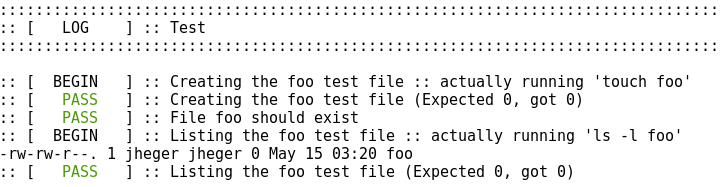
\includegraphics[width=\linewidth]{console_output.png}
  \caption{Snippet from console's output}
  \label{fig:console_output}
\end{figure}

\subsection{TESTOUT.log}
If the executed test is not connected to an \texttt{interactive shell}, the same text generated for Console's output is printed into the file \textit{TESTOUT.log}. This is mostly the case when executing a test remotely (for example in Beaker), where it is not possible to see the Console output.

\subsection{journal.xml}
Last output is a an XML\footnote{eXtensible Markup Language} file. XML is a markup language, designed to store and transport data.\cite{xml_into} 

\textit{journal.xml} is stripped off of executed commands' own output, but core information (such as which commands were executed, whether they passed or failed and so on) is kept. Also metadata about the test run (time of execution, which component was tested and more) as well as information about the hardware and software test was run on are added. \textit{journal.xml} is sent back to Beaker same as \textit{journal.txt} where it is available for further processing by automated tools. It also serves as a source of information about current state of the test during its execution, for example whether there is currently an open phase or how many failed tests or phases there are so far. Example of \textit{journal.xml} generated by Example test \ref{lst:test_example} is shown in \ref{lst:journalxml_example}.

\begin{lstlisting}[style=xml_journal,caption={Example of journal.xml},label={lst:journalxml_example}]
<?xml version="1.0"?>
<BEAKER_TEST>
  <package>basic</package>
  <pkgnotinstalled>basic</pkgnotinstalled>
  <beakerlib_rpm>beakerlib-1.15-1.fc25</beakerlib_rpm>
  <beakerlib_redhat_rpm>beakerlib-redhat-1-6.fc16</beakerlib_redhat_rpm>
  <starttime>2017-05-15 22:15:24 CEST</starttime>
  <endtime>2017-05-15 22:15:25 CEST</endtime>
  <testname>/examples/basic/Sanity/basic-test</testname>
  <release>Fedora release 25 (Twenty Five)</release>
  <hostname>localhost.localdomain</hostname>
  <arch>x86_64</arch>
  <hw_cpu>4 x Intel(R) Core(TM) i7-6600U CPU @ 2.60GHz</hw_cpu>
  <hw_ram>19496 MB</hw_ram>
  <hw_hdd>459.8 GB</hw_hdd>
  <purpose>PURPOSE of /examples/basic/Sanity/basic-test
Description: few simple commands
Author: Jakub Heger &lt;jheger@redhat.com&gt;
</purpose>
  <log>
    <phase endtime="2017-05-15 22:15:25 CEST" name="Setup" result="PASS"
score="0" starttime="2017-05-15 22:15:24 CEST" type="WARN">
      <pkgdetails sourcerpm="bash-4.3.43-4.fc25.src.rpm">bash-4.3.43-4.fc25.x86_64 </pkgdetails>
      <test message="Checking for the presence of bash rpm ">PASS</test>
      <message severity="LOG">Package versions:</message>
      <message severity="LOG">  bash-4.3.43-4.fc25.x86_64</message>
      <test command="TmpDir=$(mktemp -d)" message="Creating tmp directory (Expected 0, got 0)">PASS</test>
      <test command="pushd /tmp/tmp.mRRSJHcoBg" 
message="Command 'pushd /tmp/tmp.mRRSJHcoBg' (Expected 0, got 0)">PASS</test>
    </phase>
    <phase endtime="2017-05-15 22:15:25 CEST" name="Test" result="PASS" score="0" 
starttime="2017-05-15 22:15:25 CEST" type="FAIL">
      <pkgdetails sourcerpm="bash-4.3.43-4.fc25.src.rpm">bash-4.3.43-4.fc25.x86_64 </pkgdetails>
      <test command="touch foo" message="Creating the foo test file (Expected 0, got 0)">PASS</test>
      <test message="File foo should exist ">PASS</test>
      <test command="ls -l foo" message="Listing the foo test file (Expected 0, got 0)">PASS</test>
    </phase>
    <phase endtime="2017-05-15 22:15:25 CEST" name="Cleanup" result="PASS" score="0" 
starttime="2017-05-15 22:15:25 CEST" type="WARN">
      <pkgdetails sourcerpm="bash-4.3.43-4.fc25.src.rpm">bash-4.3.43-4.fc25.x86_64 </pkgdetails>
      <test command="popd" message="Command 'popd' (Expected 0, got 0)">PASS</test>
      <test command="rm -r /tmp/tmp.mRRSJHcoBg" 
message="Removing tmp directory (Expected 0, got 0)">PASS</test>
    </phase>
    <message severity="LOG">JOURNAL XML: /var/tmp/beakerlib-SJCxN82/journal.xml</message>
    <message severity="LOG">JOURNAL TXT: /var/tmp/beakerlib-SJCxN82/journal.txt</message>
  </log>
</BEAKER_TEST>
\end{lstlisting}

\subsection{BeakerLib directory}
\label{beakerlib_dir}
Described files are saved into a BeakerLib test directory created for each individual test. 

If the test is run locally, temporary directory is created on system with \texttt{mktemp} command, which creates pseudo-random name.

If run on Beaker a unique \textbf{TESTID} is generated for each test. This ID serves as a name for test directory as well as an identifier which Beaker later uses when connecting test results with correct test. It is also important in case where restart is a regular part of a test. Upon restarting the test machine the same \textbf{TESTIDs} are relayed from Beaker to Harness with information which tests were already run. Harness then continues with execution of unfinished tests, starting with test that caused the restart, in the same BeakerLib directory it did before, where there are partial results of the test, so it can continue where it left off.


\section{Source files}
This section describes a few of BeakerLib's source files, relevant to this thesis.
\begin{itemize}
\item \textit{beakerlib.sh} - Starting point of every tests. It is \texttt{sourced} at the beginning of each test and in turn \texttt{sources} all other BeakerLib files.
\item \textit{testing.sh} - Contains definitions of the most used \textbf{rlCommands} as well as some internal functions.
\item \textit{journal.sh} - Provides bash-side Journaling functionality. Functions from this file process information about what to log and relay them to \textit{journalling.py}.
\item \textit{journalling.py} - Python script responsible for creating most of BeakerLib's outputs. It also creates and modifies \textit{journal.xml} file.
\end{itemize}

\section{Analysis of slow performance}
It was reported that BeakerLib suffers performance problems when running long tests. Time of processing each \textbf{rlCommand} grew longer after many (several hundreds and more) were used. Analysis of library was problematic due to lack of documentation, complex structure and uncommented code, however thorough investigation of the source code indicated that problem lies with generating \textit{journal.xml}. 

Python script \textit{journalling.py} is called after each \textbf{rlCommand} to log its result into \textit{journal.xml}. This isn't big problem with small test as the \textit{journal.xml} file takes up only a few kilobytes, however when the file takes up dozens or hundreds of kilobytes, repeated loading the file from disk, parsing, adding a line of log and then saving the file back to the disk adds significantly more load to CPU\footnote{Central Processing Unit}. Running larger tests therefore becomes quite time consuming and considerably slows down testing as a whole.

This has been determined as the main focus of the thesis since it probably is the most significant performance bottleneck. The next chapter describes proposed solutions with their pros and cons.

Figure \ref{fig:rl_run} illustrates simplified version of how \textbf{rlRun} propagates through different functions from BeakerLib files (which are \texttt{sourced} at the time test execution,  depicted by rounded rectangles) and how it is logged into the Journal. Similar operation is performed for every \textbf{rlCommand} in a test.

\begin{figure}[h!]
  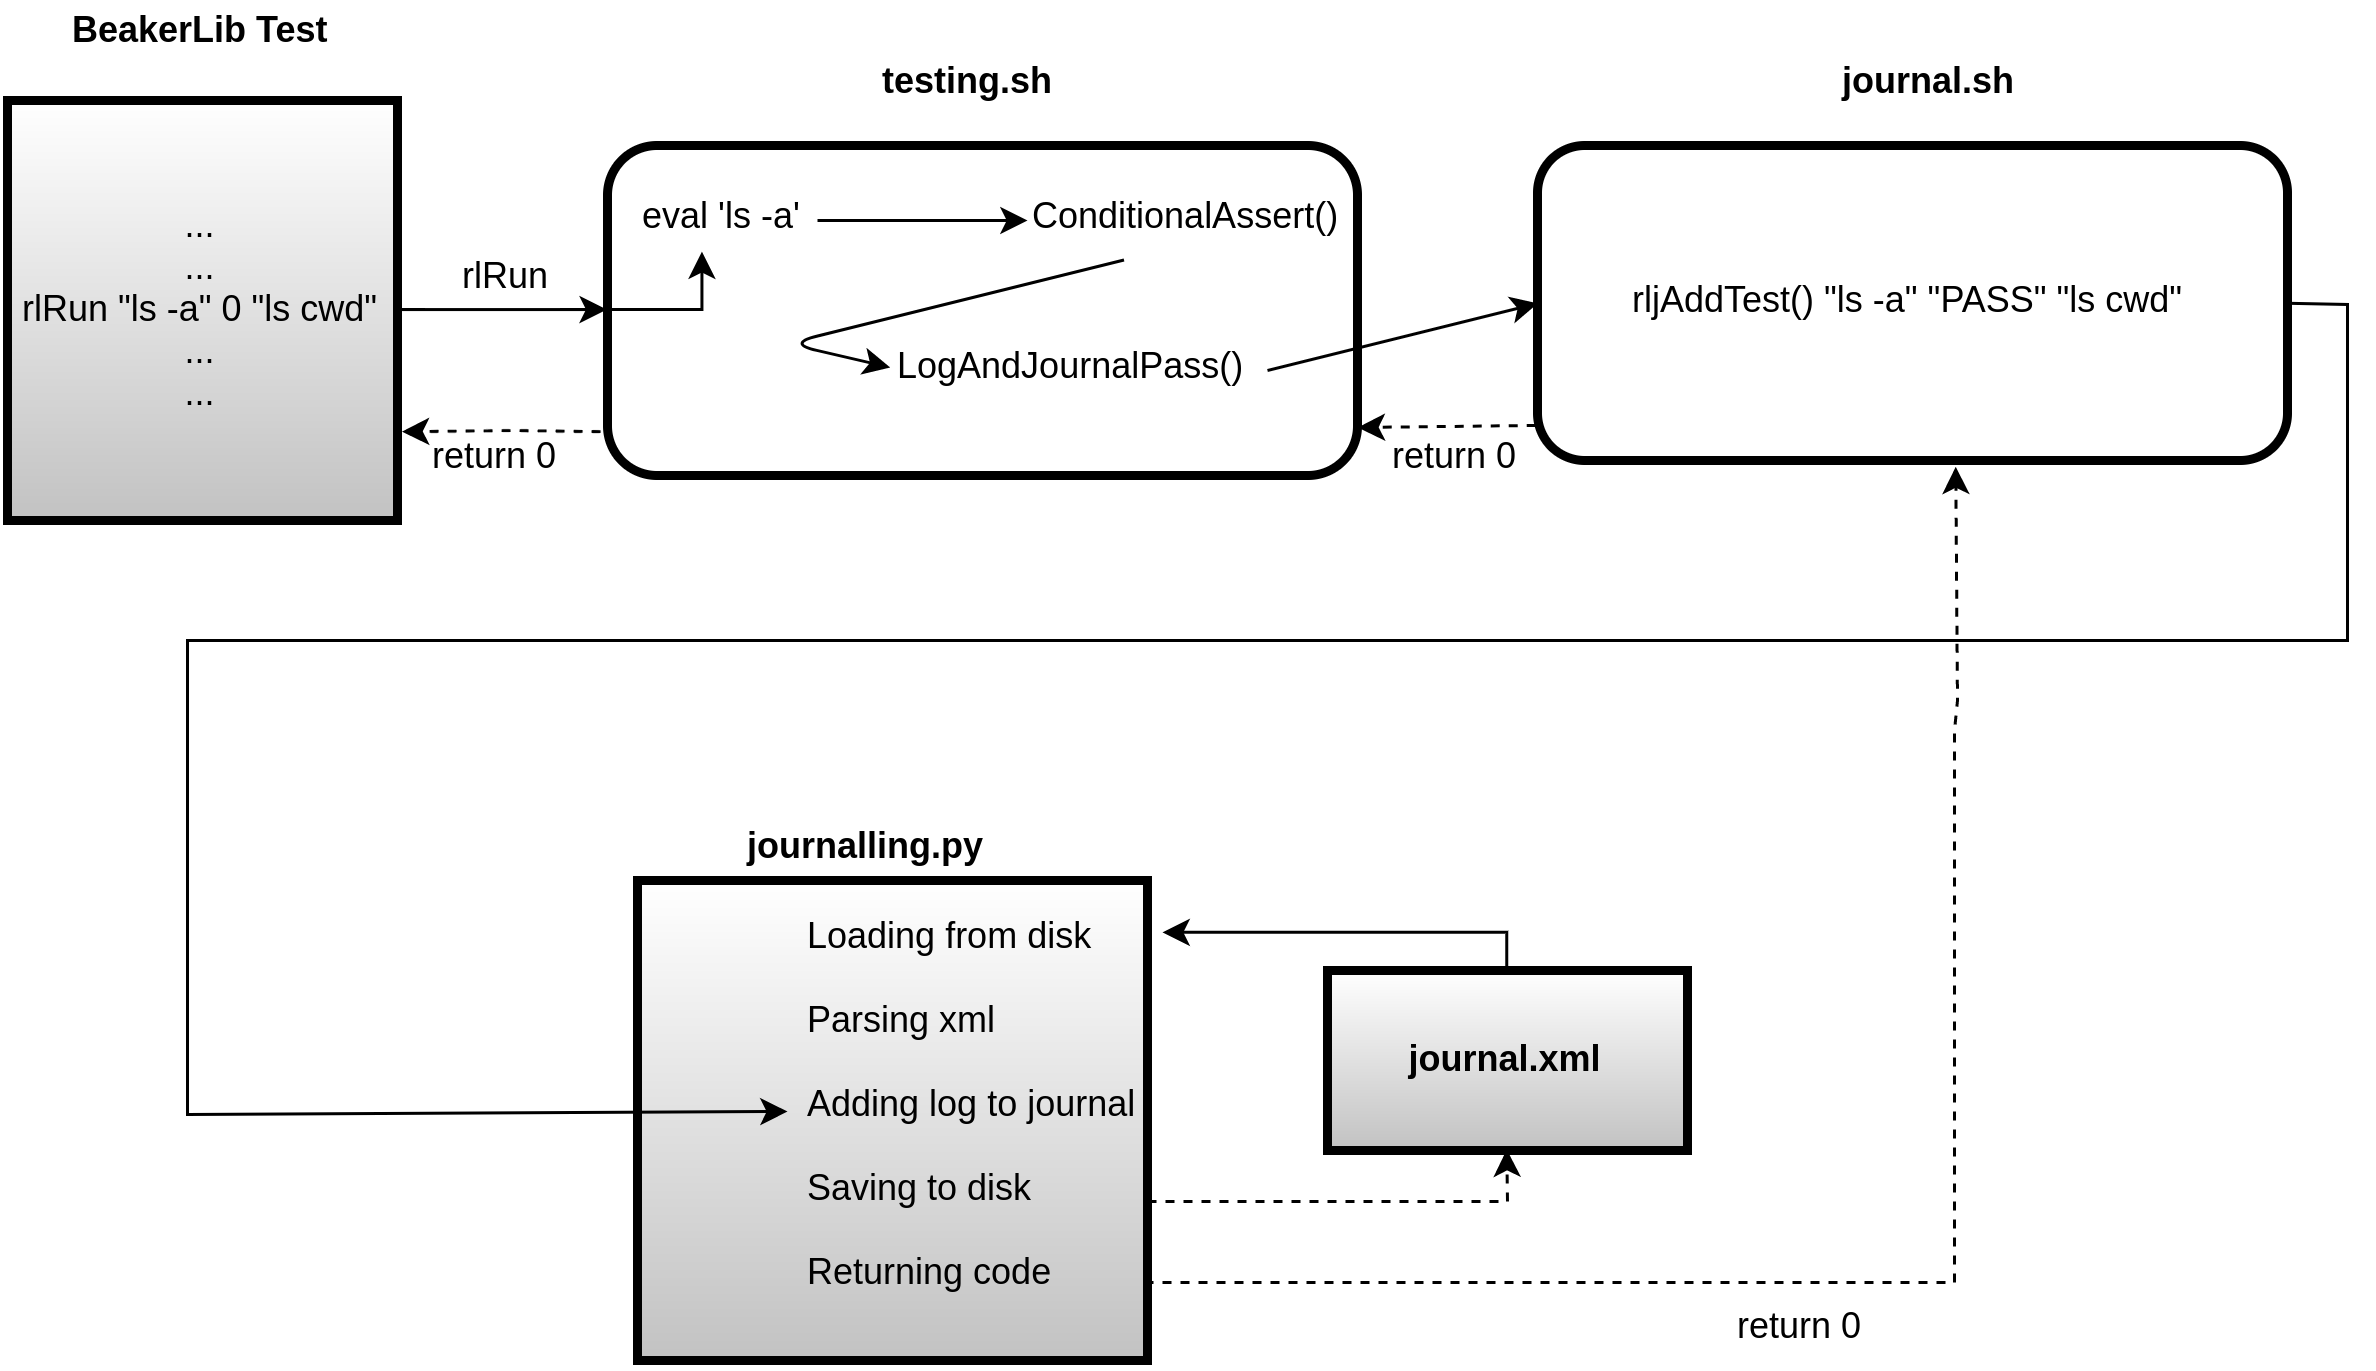
\includegraphics[width=\linewidth]{rl_run.png}
  \caption{Logging of rlRun to Journal}
  \label{fig:rl_run}
\end{figure}

\chapter{Solution of Journaling problem}
\label{solutions}

Sections in this chapter provide possible solutions to the Journaling problem. Besides explaining the principle of each solution, the sections also discuss their advantages, disadvantages and potential issues.

\section{Change of xml parser}
XML parser is a program which can turn XML document into structured object in RAM\footnote{Random Access Memory}. Depending on implementation of the parser, that object is then easier to access by the program as it may provide methods to navigate the object and search it or potentially modify. 

Parsing of XML in BeakerLib is done by \textit{journalling.py} script by \texttt{Python} module \texttt{xml.dom.minidom}\cite{minidom_doc}. 

 \texttt{xml.dom.minidom} is a native part of \texttt{Python} from version 2.0 and provides minimal implementation of the DOM\footnote{Document Object Model} interface, with an API\footnote{Application Programming Interface} similar to that in other languages. 

I decided to change parser to different one, to measure whether it will provide better performance. Because of reasons of backward compatibility with RHEL 5\footnote{Red Hat Enterprise Linux 5} which needs to be supported by BeakerLib, the choice of XML parsers was limited to native modules of \texttt{Python 2.4.3}. Two additional XML parsers were present for given version.

\begin{itemize}
\item lxml - The \texttt{lxml} XML toolkit is a Pythonic binding for the C libraries libxml2 and libxslt. It combines the speed and XML feature completeness of these libraries with the simplicity of a native \texttt{Python} API.  \cite{lxml_doc}

It works similarly to \texttt{xml.dom.minidom} in the way that when reading XML object from a file, it will read it whole, builds an object out of it and provides methods for the object to allow access to it.
\item xml.sax  \cite{sax_doc} - \texttt{xml.sax} originated as a parser for \texttt{Java}\cite{Sax2}. In \texttt{Python} it was released with version 2.0. It differs from \texttt{xml.dom.minidom} and \texttt{lxml} where the two mentioned parsers work with a whole XML file,  \texttt{xml.sax} emits events as it goes step by step through the file\cite{sax_example}. Using this approach means less memory has to be allocated for XML handling and therefore makes it ideal when working with very large amount of XML  data.
\end{itemize}

I decided to implement \texttt{lxml} parser as it is supposed to be faster and less demanding on memory than \texttt{xml.dom.minidom}\cite{lxml_performance}, while keeping its intuitive interface.

\section{Change in calling journalling.py}
Next proposition to make BeakerLib faster is in a way \textit{journalling.py} is called. The assumption being that repeated parsing of XML document slows BeakerLib the most, reducing the number of times it was parsed was then the highest priority. 

\subsection{Queue file solution}
First solution is to create a new, temporary \textbf{queue file}, which will act as a kind of buffer. \mbox{\textbf{rlCommands}} will behave as before apart from creating BeakerLib journals, but instead they will write message into the \textbf{queue file}. This file will be read and processed only when necessary, that is at the end each phase, when journals are sent to Beaker.

\subsubsection{Disadvantages}
The way BeakerLib is designed now it in most cases expects some form of return value from \textit{journalling.py} immediately after adding a log to a journal. Performed logging either returns code indicating success of failure or \texttt{string} with information about the current state of test. This presents problem as there is no way how to communicate back these information when parsing is postponed. 

\subsection{Daemon-like solution}
Second solution is to rewrite \textit{journalling.py} script to have daemon-like behavior. That is to have it run as its own process throughout the whole time of test execution. The XML object will be stored in memory, and parsed as whole only at the beginning of journal creation and in case of restarting the test run (which happen when machine is rebooted).  

This way BeakerLib can receive response about current test state immediately while still keeping CPU load minimal. Daemon-like solution however brings different obstacles.

\subsubsection{Disadvantages}
An independent, potentially long running process daemon is more prone to unplanned events such as unexpected exit. This must be addressed by both daemon (to exit as safely as possible)  and by the rest of BeakerLib (to detect that daemon is no longer running and to behave accordingly). 

\subsubsection{Communication}
Inter-process communication between running test and daemon has to be created for test to inform which \textbf{rlCommand} is supposed to be logged and for daemon to respond with current state of XML document. This two-way communication must be synchronous to assure BeakerLib and daemon process their respective messages in correct order. I considered following options:

\begin{itemize}
\item Unix sockets  -  <expand>
\item Named pipes - Named pipes are device files. They allow inter-process communication by reading it and writing into is as if regular file, however under normal circumstances the read/write is a blocking operation\cite{pipes_blocking}. This means if one process opens pipe for reading, it will hang there until another process opens the pipe for writing. This feature can be used for synchronization of communication between processes. 
\end{itemize}

% DOPLINT CITACE ^^ ???

I chose to implement communication through Named pipes because synchronization issue is taken care of because of the way Named pipes are designed.


\chapter{Implementation of proposed solutions}
\label{implementations}
This chapter describes how the proposed solutions were implemented. Each solution has its own section that describes implementation details and obstacles that were found and had to be solved during the implementation.
During changing of parsers I discovered and fixed few bugs present in current implementation of \textit{journalling.py}.

\section{Change of xml parser}
\subsection{Difference in parsers}
As mentioned before I chose to change original XML parser to \texttt{lxml}. Only changes in code were in file \textit{journalling.py} as it is only part of BeakerLib that directly works with journal's XML object. 
Most of the changes consisted in changing \texttt{xml.dom.minidom's} method for creating new XML element and assigning value into it.
Biggest difference between given parsers is that \texttt{lxml} does not provide many helping methods as \texttt{xml.dom.minidom} does.
For example in \texttt{lxml}  there is no method \texttt{getElementsByTagName()} to search XML object by a tag name. Instead \texttt{lxml} supports \texttt{xpath} \cite{xpath} syntax for searching the object. xpath\footnote{XML Path Language} is part of XSLT\footnote{eXtensible Stylesheet Language Transformations} standard. It be can used to navigate through elements and attributes in an XML document.

Another example of difference is an approach for accessing element's children. While \texttt{xml.dom.minidom} has dedicated methods and attributes such as \texttt{hasChildNodes()} which returns \texttt{bool} value or \texttt{childNodes} which is a iterable attribute of element's children, \texttt{lxml} has more low level implementation. It treats elements as python lists so \texttt{hasChildNodes()} can be replaced with simple \texttt{len(element) != 0}.
\\
\\
Because preliminary performance measurement showed faster test execution with \texttt{lxml}, I decided to implement the rest of the proposed solutions with this parser.

\section{Queue file solution}
This section deals with implementation of \textbf{queue file} solution. It is divided into subsections that discuss files I designed or changed during implementation. 

\subsection{Queue file}
\textbf{Queue file} was designed in a way so it was simple to implement, in a human readable format for potential test debugging and easy to extend by new, future functions that will work with it. 
It is a plain text file, each line containing one buffered command for \texttt{Python} script to process later, on demand. 

\subsection{journal.sh}
Creation of  \textbf{queue file}, by using \texttt{touch} command, was added to function \texttt{rlJournalStart()} which initializes Journaling functionality. Using \texttt{touch} assures that if the \textbf{queue file} already exists (which happens when test run is interrupted and started again), its content is not deleted (in case of restart of the testing machine as described in section \ref{beakerlib_dir}).

It now also \texttt{exports} new variable \textbf{BEAKERLIB\_QUEUE}, with \textbf{queue file's} path, into test's environment so \texttt{Python} script \textit{od\_journalling.py}, can later access it.

Original calling of \textit{journalling.py} script, which is a main functionality of \textit{journal.sh}, was replaced in one of two ways:

\begin{itemize}
\item Delayed calling - New function \texttt{rljPrintToQueue()} takes all arguments that were originally meant for \textit{journalling.py} and instead prints them into \textbf{queue file}, where it will be processed by \textit{od\_journalling.py} later during execution of the test. This concerns functions which do not necessary require response about current test state from \textit{journal.xml}.  Namely functions: \texttt{rlJournalPrint()}, \texttt{rljAddTest()}, \texttt{rljAddMetric()}, \texttt{rljAddMessage()}, \texttt{rljRpmLog()}
\item Immediate calling of \textit{od\_journalling.py} - Virtually the same as the original solution. These functions require immediate response. Using this way of calling won't save on any CPU load (in fact the the load will be slightly higher than before because of operations related to \textbf{queue file} processing), however in typical BeakerLib test these functions are in minority compared to previous type of calling.  Functions and the response they require are:  
\begin{itemize}
\item \texttt{rlJournalStart()} - requires confirmation that journal was initiated successfully
\item \texttt{rlJournalPrintText()} - requires \textit{journal.txt} which is generated from current \mbox{\textit{journal.xml}}
\item \texttt{rlGetTestState()}  - requires number of failed asserts in the test so far
\item \texttt{rlGetPhaseState()} - requires number of failed phases in the test so far
\item \texttt{rljAddPhase()} - requires immediate print
\item \texttt{rljClosePhase()} - requires result of closed phase, to send it to Beaker along with Journal
\item \texttt{rlJournalStart()}
\end{itemize}
\end{itemize}

Function \texttt{rljAddTest()} is the cause of the most calls of \textit{journalling.py} in original solution, therefore had the highest need to be moved into group of functions with Delayed calling. However it does require knowledge of current state of the test. That being situation when Assert (rlCommand using \texttt{rljAddTest()} for Journaling) is used outside of a phase, such information is held only in current \textit{journal.xml}. To solve this problem functionality of  \texttt{rljAddTest()} had to moved into \textit{{od\_journalling.py}} script, discussed in the next subsection.

Apart from printing to \textbf{queue file}, \texttt{rljPrintToQueue()} also has to escape given arguments. This done because firstly some of the arguments originating from user may contain newline character which would break the"one buffered command per line" rule in  \textbf{queue file's} format and secondly so \textit{od\_journalling.py} may parse it with \texttt{optparse} module.
Escaping is done with \texttt{printf} bash builtin\cite{bash_builtins}, specifically its \texttt{\%q} option which causes \texttt{printf} to output in \texttt{shell-quoted} format.

\subsection{od\_journalling.py}
File \textit{od\_journalling.py} originated from \textit{journalling.py} but it differs in some ways.

Now when it is called, it first parses current \textit{journal.xml} and then calls new method \texttt{updateXML()} with parsed XML object as an argument. This method opens \textbf{queue file} and finds last line it accessed in previous call. From there it reads buffered lines, and modifies the XML object accordingly in the similar way it did originally, this time however without parsing \textit{journal.xml} each time as the XML object is passed as an argument to appropriate methods. 

When it reaches end of file, it makes a mark for future readings and returns to the original call coming from one of the \textit{journal.sh's}  Immediate calling functions. After modification from that function it generates response and returns it to \textit{journal.sh}. 

Exceptions to this behavior are calls  from \texttt{rlJournalStart()}, which doesn't access \textbf{queue file} but only initializes XML object and returns exit code whose value depends on how was initialization successful and \texttt{rlJournalEnd()} which makes sure every buffered command was processed as it is an exit point from the test.

As mentioned in previous subsection, functionality of  \texttt{rljAddTest()} had to be altered. Given that bash side of BeakerLib had no way of knowing if the test was added outside of phase at the time of writing this operation into the \textbf{queue file}, this action had to be resolved when \textit{od\_journalling.py} processed the \textbf{queue file}. 
New method \texttt{testOutOfPhase()} was implemented which is called when assertion outside of phase is detected and it performs the same process as when this event happened in original \textit{journal.sh}.

\subsection{Problems with implementation}
Main goal of this solution was to reduce number of times \textit{journal.xml} is parsed, by delaying as many Journaling operations as possible, while keeping BeakerLib's outputs the same. The way BeakerLib is designed now it is not possible, because some information is always lost when operations are delayed. In case of this implementation I was able to keep \textit{journal.xml}, and therefore \textit{journal.txt}  as well, the same as with original solution, however at the price Console's output which is now missing some information usually given by functions from Delayed calling category.

Solving this issue would require more extensive changes to BeakerLib's design which I decided not to implement for now so \textbf{Queue file} solution remains only as a proof of concept.

\section{Daemon-like solution}
This section is divided into subsections which describe individual changes I made to BeakerLib's design.

\subsection{journal.sh}
Function \texttt{rlJournalStart()} in this implementation creates Named pipe using \texttt{mkfifo} and then \texttt{exports} its path into environment.
Then it spawns \textit{daemon\_journalling.py} process in the background with \texttt{\&} operator and store its \texttt{PID\footnote{Process identifier}}.

Every call of \textit{journalling.py} in original implementation was replace with new function \texttt{rljCallDaemon()}, which takes the same arguments as original function. When this new function is called it firstly escapes given arguments using similar way as in \textbf{queue file}, this time however another function had to be created.  \texttt{rljCallDaemon()} passes its argument to the function \texttt{escapeArguments()} which uses \texttt{printf} and \texttt{echo} bash builtins to escape arguments in loop which are then caught back in \texttt{rljCallDaemon()} with \texttt{\$()} construct\cite{command_substitution} for catching output. It is implemented this way to avoid using temporary file.

After arguments are escaped, \texttt{rljCallDaemon()} checks whether the Daemon is still running with \texttt{kill -0 \$DAEMON\_PID} call. 

\texttt{kill} program is used to send signals to processes. If used with \texttt{-0} option, no signal is actually sent but error checking against the process is still performed and it returns \texttt{0} when process with given PID is running\cite{man_kill}. This is done to make sure the Daemon is still running before pipe writing operation.  If the Daemon wasn't running before writing to pipe, the test would hang there indefinitely, so if the Daemon is not running, the test exits with error.

After this check is performed, \texttt{rljCallDaemon()} writes to Named pipe its escaped message, where it wait until Daemon responds. Response is read as a next action, decoded from a format that will discussed later and then response is returned to function that called \texttt{rljCallDaemon()}. 
This is repeated until end of the test is reached.

\subsection{Daemon}
\textit{journalling\_daemon.py} script again originates from \textit{journalling.py}. This time however it designed to run in continuous loop, instead of closing after one executed action.

\section{testing that my solution is the same}

\chapter{Performance measuring}
\label{performance}
<Definition of performance measuring>

For performance measuring of BeakerLib I chose two kinds of tests in in two kinds of testing environments.

\section{Tests}

\subsection{Artificial tests}
First type of tests are artificial tests created by me with \texttt{beaker-wizard} tool to specifically target and measure performance of journaling modifications I made. They consist mostly of \textbf{rlCommands} that directly work with \texttt{journalling.py}. For example commands \textbf{rlLog} or \textbf{rlPhaseStart} and \textbf{rlPhaseEnd}. This way we can observe clear difference in performance without being affected by operations unrelated to journaling (executing actions that verify functionality of components in real tests). 

<description of artificial tests with links to Appendix>

\subsection{Real tests}
Second type are real tests used in Red Hat. These are examples of tests that have been reported to have bad performance with BeakerLib so I am testing them to see if my modifications have real life impact on performance.

<description of real tests>

\section{Testing Environment}

\subsection{Local}
First environment is local laptop for convenience and speed of execution. Tests were run directly, without any harness and with these technical specifications. 

<table of tech specs>

\subsection{Remote in beaker}
Second round of testing was done to emulate real testing conditions and to verify that changes made to BeakerLib do not break functionality outside of controlled environment. Tests were run with the default test harness Beah.
<table of tech specs>

\section{Measured Values}

\section{Baseline measurements}
<results>


\section{Implemented optimizations}
<results>

\chapter{Analysis of results}
\label{results}

\chapter{Conclusion}
\label{conclusion}
Recap of results
\\
Future work


%=========================================================================
 % viz. obsah.tex / see obsah.tex

  % Pouzita literatura / Bibliography
  % ----------------------------------------------
%\ifslovak
  %\makeatletter
  %\def\@openbib@code{\addcontentsline{toc}{chapter}{Literatúra}}
  %\makeatother
 % \bibliographystyle{bib-styles/czechiso}
%\else
  %\ifczech
    %\makeatletter
    %\def\@openbib@code{\addcontentsline{toc}{chapter}{Literatura}}
    %\makeatother
   % \bibliographystyle{bib-styles/czechiso}
  %\else 
    \makeatletter
    \def\@openbib@code{\addcontentsline{toc}{chapter}{Bibliography}}
    \makeatother
    \bibliographystyle{bib-styles/englishiso}
    %\bibliographystyle{alpha}
 % \fi
%\fi
  \begin{flushleft}
  \bibliography{projekt-20-literatura-bibliography}
  \end{flushleft}

  % vynechani stranky v oboustrannem rezimu
  % Skip the page in the two-sided mode
  \iftwoside
    \cleardoublepage
  \fi

  % Prilohy / Appendices
  % ---------------------------------------------
  \appendix
\ifczech
  \renewcommand{\appendixpagename}{Přílohy}
  \renewcommand{\appendixtocname}{Přílohy}
  \renewcommand{\appendixname}{Příloha}
\fi
\ifslovak
  \renewcommand{\appendixpagename}{Prílohy}
  \renewcommand{\appendixtocname}{Prílohy}
  \renewcommand{\appendixname}{Príloha}
\fi
  \appendixpage

% vynechani stranky v oboustrannem rezimu
% Skip the page in the two-sided mode
\iftwoside
  \cleardoublepage
\fi
  
%\ifslovak
%  \section*{Zoznam príloh}
%  \addcontentsline{toc}{section}{Zoznam príloh}
%\else
 % \ifczech
%    \section*{Seznam příloh}
%    \addcontentsline{toc}{section}{Seznam příloh}
 % \else
    \section*{List of Appendices}
    \addcontentsline{toc}{section}{List of Appendices}
  %\fi
%\fi
  \startcontents[chapters]
  % seznam příloh / list of appendices
   \printcontents[chapters]{l}{0}{\setcounter{tocdepth}{2}}
  
  % vynechani stranky v oboustrannem rezimu
  \iftwoside
    \cleardoublepage
  \fi
  % Tento soubor nahraďte vlastním souborem s přílohami (nadpisy níže jsou pouze pro příklad)
% This file should be replaced with your file with an appendices (headings below are examples only)

% Umístění obsahu paměťového média do příloh je vhodné konzultovat s vedoucím
% Placing of table of contents of the memory media here should be consulted with a supervisor
%\chapter{Obsah přiloženého paměťového média}

%\chapter{Manuál}

%\chapter{Konfigurační soubor} % Configuration file

%\chapter{RelaxNG Schéma konfiguračního souboru} % Scheme of RelaxNG configuration file

%\chapter{Plakát} % poster

\chapter{Content of enclosed CD}
\label{appendix:cd}
Files:
\begin{itemize}
  \item \textbf{pdf} - PDF version of the thesis
\end{itemize}

\chapter{Measured values}
\label{appendix:data}

\section{Baseline measurements}

\subsubsection{Local}

\begin{center}
\scalebox{0.8}{
    \begin{tabular}{| c | c | c | c | c | c | c | c | c | c | c | c | c | c | c | c | c | c | c | c |}
    \hline
    Test & \multicolumn{15}{|c|}{Measured time is seconds} & Average \\ \hline

Test1 & 1 & 1 & 1 & 1 & 1 & 1 & 0 & 1 & 1 & 1 & 1 & 0 & 1 & 1 & 1 & 0.9 \\ \hline
Test2 & 62 & 63 & 63 & 64 & 67 & 66 & 63 & 63 & 66 & 65 & 65 & 63 & 64 & 64 & 61 & 63.9 \\ \hline
Test3 & 109 & 109 & 110 & 110 & 112 & 110 & 119 & 112 & 113 & 111 & 114 & 111 & 118 & 110 & 109 & 111.8 \\ \hline
Test4 & 393 & 396 & 397 & 408 & 398 & 395 & 400 & 421 & 429 & 407 & 395 & 398 & 399 & 395 & 403 & 402.3 \\ \hline
Test5 & 45 & 46 & 43 & 47 & 42 & 42 & 43 & 42 & 42 & 42 & 42 & 42 & 42 & 43 & 43 & 43.1 \\ \hline
Test6 & 4 & 5 & 4 & 3 & 3 & 3 & 4 & 4 & 5 & 3 & 4 & 4 & 3 & 3 & 2 & 3.6 \\ \hline
    \end{tabular}
}
\end{center}



\subsubsection{Remote}

\begin{center}
\scalebox{0.8}{
    \begin{tabular}{| c | c | c | c | c | c | c | c | c | c | c | c | c | c | c | c | c | c | c | c |}
    \hline
    Test & \multicolumn{15}{|c|}{Measured time is seconds} & Average \\ \hline
    Test1 & 27 & 21 & 19 & 22 & 19 & 19 & 19 & 20 & 20 & 20 & 19 & 19 & 19 & 19 & 20 & 21.1 \\ \hline
    Test 2 & 132 & 125 & 127 & 122 & 122 & 122 & 122 & 121 & 121 & 125 & 120 & 123 & 124 & 122 & 126 & 123.6 \\ \hline
    Test 3 & 1239 & 1303 & 1241 & 1258 & 1274 & 1282 & 1295 & 1289 & 1307 & 1285 & 1293 & 1296 & 1295 & 1303 & 1312 & 1284.8\\ \hline
    Test 4 & 1417 & 1400 & 1390 & 1383 & 1535 & 1501 & 1548 & 1413 & 1490 & 1531 & 1541 & 1455 & 1437 & 1487 & 1402 & 1462  \\ \hline
    Test 5 & 313 & 189 & 184 & 180 & 182 & 178 & 181 & 182 & 182 & 181 & 180 & 184 & 182 & 178 & 180 &  190.4\\ \hline
    Test 6 & 85 & 40 & 40 & 41 & 38 & 38 & 40 & 46 & 39 & 39 & 39 & 39 & 38 & 39 & 40 & 42.7 \\ \hline
    \end{tabular}
}
\end{center}

\section{Implemented optimizations}

\subsection{lxml parser}

\subsubsection{Local}

\begin{center}
\scalebox{0.8}{
    \begin{tabular}{| c | c | c | c | c | c | c | c | c | c | c | c | c | c | c | c | c | c | c | c |}
    \hline
    Test & \multicolumn{15}{|c|}{Measured time is seconds} & Average \\ \hline
Test1 & 1 & 1 & 2 & 1 & 1 & 1 & 1 & 2 & 1 & 1 & 2 & 1 & 1 & 1 & 1 & 1.2 \\ \hline
Test2 & 61 & 60 & 65 & 63 & 62 & 61 & 61 & 61 & 63 & 60 & 60 & 62 & 63 & 61 & 59 & 61.5 \\ \hline
Test3 & 100 & 88 & 88 & 88 & 96 & 96 & 96 & 97 & 98 & 101 & 98 & 96 & 97 & 98 & 100 & 95.8 \\ \hline
Test4 & 228 & 228 & 236 & 236 & 241 & 246 & 236 & 219 & 214 & 214 & 211 & 208 & 206 & 222 & 231 & 225.1 \\ \hline
Test5 & 46 & 46 & 45 & 46 & 46 & 46 & 47 & 45 & 47 & 46 & 47 & 47 & 46 & 48 & 46 & 46.3 \\ \hline
Test6 & 6 & 6 & 6 & 5 & 5 & 5 & 5 & 5 & 5 & 6 & 5 & 5 & 5 & 3 & 6 & 4.9 \\ \hline
    \end{tabular}
}
\end{center}

\subsubsection{Remote}

\begin{center}
\scalebox{0.8}{
    \begin{tabular}{| c | c | c | c | c | c | c | c | c | c | c | c | c | c | c | c | c | c | c | c |}
    \hline
    Test & \multicolumn{15}{|c|}{Measured time is seconds} & Average \\ \hline
    Test1 & 25 & 19 & 19 & 19 & 19 & 20 & 20 & 19 & 20 & 20 & 20 & 19 & 19 & 19 & 20 & 19.8 \\ \hline
    Test2 & 121 & 113 & 113 & 113 & 113 & 113 & 113 & 115 & 114 & 115 & 114 & 114 & 113 & 113 & 113 & 114 \\ \hline
    Test3 & 1322 & 1223 & 1247 & 1264 & 1261 & 1281 & 1290 & 1292 & 1301 & 1286 & 1293 & 1293 & 1295 & 1302 & 1304 & 1283.6 \\ \hline
    Test4 & 1042 & 1035 & 1036 & 1109 & 1097 & 1049 & 1039 & 1033 & 1037 & 1039 & 1040 & 1037 & 1036 & 1035 & 1037 & 1046.7  \\ \hline
    Test5 & 302 & 180 & 175 & 175 & 175 & 176 & 176 & 176 & 177 & 178 & 175 & 176 & 180 & 172 & 175 & 184.5 \\ \hline
    Test6 & 75 & 37 & 36 & 36 & 36 & 37 & 37 & 37 & 38 & 36 & 36 & 43 & 37 & 37 & 36 & 39.6 \\ \hline
    \end{tabular}
}
\end{center}

\subsection{Queue file solution with lxml parser}

\subsubsection{Local}

\begin{center}
\scalebox{0.8}{
    \begin{tabular}{| c | c | c | c | c | c | c | c | c | c | c | c | c | c | c | c | c | c | c | c |}
    \hline
    Test & \multicolumn{15}{|c|}{Measured time is seconds} & Average \\ \hline
Test1 & 0 & 0 & 0 & 0 & 1 & 1 & 1 & 1 & 1 & 0 & 0 & 0 & 0 & 0 & 0 & 0.3 \\ \hline
Test2 & 4 & 4 & 3 & 4 & 5 & 4 & 4 & 4 & 4 & 4 & 4 & 4 & 4 & 4 & 4 & 4 \\ \hline
Test3 & 101 & 102 & 105 & 97 & 98 & 99 & 101 & 97 & 100 & 99 & 98 & 98 & 97 & 103 & 99 & 99.6 \\ \hline
Test4 & 119 & 119 & 116 & 117 & 121 & 117 & 116 & 117 & 118 & 124 & 116 & 115 & 116 & 116 & 107 & 116.9 \\ \hline
Test5 & 12 & 11 & 12 & 12 & 11 & 12 & 12 & 12 & 12 & 12 & 12 & 12 & 12 & 12 & 12 & 11.9 \\ \hline
Test6 & 2 & 2 & 2 & 2 & 2 & 1 & 2 & 1 & 1 & 2 & 2 & 1 & 1 & 2 & 1 & 1.6 \\ \hline
    \end{tabular}
}
\end{center}

\subsubsection{Remote}

\begin{center}
\scalebox{0.8}{
    \begin{tabular}{| c | c | c | c | c | c | c | c | c | c | c | c | c | c | c | c | c | c | c | c |}
    \hline
    Test & \multicolumn{15}{|c|}{Measured time is seconds} & Average \\ \hline
    Test1 & 27 & 19 & 19 & 20 & 20 & 19 & 19 & 20 & 19 & 19 & 20 & 20 & 19 & 20 & 20 & 20 \\ \hline
    Test2 & 27 & 22 & 22 & 22 & 22 & 21 & 21 & 21 & 21 & 21 & 21 & 21 & 21 & 22 & 22 & 21.8 \\ \hline
    Test3 & 1316 & 1227 & 1254 & 1259 & 1276 & 1283 & 1288 & 1292 & 1281 & 1291 & 1289 & 1293 & 1292 & 1307 & 1305 & 1283.5 \\ \hline
    Test4 & 898 & 890 & 881 & 875 & 876 & 877 & 871 & 910 & 994 & 957 & 977 & 935 & 880 & 913 & 935 & 911.3  \\ \hline
    Test5 & 249 & 130 & 133 & 134 & 130 & 134 & 131 & 136 & 133 & 133 & 133 & 133 & 132 & 129 & 131 & 140.1 \\ \hline
    Test6 & 86 & 45 & 39 & 36 & 36 & 36 & 36 & 37 & 36 & 43 & 36 & 38 & 37 & 35 & 36 & 40.8 \\ \hline
    \end{tabular}
}
\end{center}

\subsection{Daemon solution with  lxml parser}

\subsubsection{Local}

\begin{center}
\scalebox{0.8}{
    \begin{tabular}{| c | c | c | c | c | c | c | c | c | c | c | c | c | c | c | c | c | c | c | c |}
    \hline
    Test & \multicolumn{15}{|c|}{Measured time is seconds} & Average \\ \hline
Test1 & 1 & 0 & 0 & 1 & 0 & 0 & 1 & 0 & 0 & 1 & 0 & 0 & 1 & 0 & 0 & 0.3 \\ \hline
Test2 & 5 & 6 & 6 & 6 & 6 & 6 & 5 & 5 & 5 & 6 & 5 & 6 & 6 & 7 & 7 & 5.8 \\ \hline
Test3 & 20 & 20 & 21 & 21 & 20 & 20 & 19 & 22 & 21 & 21 & 20 & 21 & 20 & 24 & 20 & 20.7 \\ \hline
Test4 & 44 & 44 & 44 & 44 & 44 & 44 & 45 & 42 & 42 & 44 & 46 & 45 & 45 & 46 & 44 & 44.2 \\ \hline
Test5 & 13 & 13 & 13 & 13 & 13 & 13 & 13 & 13 & 13 & 12 & 13 & 13 & 13 & 13 & 13 & 12.9 \\ \hline
Test6 & 14 & 14 & 14 & 14 & 14 & 14 & 14 & 14 & 14 & 14 & 14 & 14 & 15 & 14 & 14 & 14.1 \\ \hline
    \end{tabular}
}
\end{center}

\subsubsection{Remote}

\begin{center}
\scalebox{0.8}{
    \begin{tabular}{| c | c | c | c | c | c | c | c | c | c | c | c | c | c | c | c | c | c | c | c |}
    \hline
    Test & \multicolumn{15}{|c|}{Measured time is seconds} & Average \\ \hline
    Test1 & 27 & 21 & 19 & 22 & 19 & 19 & 19 & 20 & 20 & 20 & 19 & 19 & 19 & 19 & 20 & 21.1 \\ \hline
    Test2 & 40 & 41 & 32 & 37 & 43 & 30 & 32 & 28 & 29 & 55 & 55 & 33 & 42 & 29 & 27 & 36.9 \\ \hline
    Test3 & 1249 & 1226 & 1243 & 1256 & 1271 & 1294 & 1278 & 1292 & 1287 & 1286 & 1283 & 1283 & 1290 & 1304 & 1308 & 1276.7 \\ \hline
    Test4 & 773 & 780 & 787 & 751 & 814 & 745 & 731 & 736 & 783 & 757 & 759 & 787 & 741 & 732 & 736 & 760.8  \\ \hline
    Test5 & 238 & 129 & 125 & 124 & 125 & 122 & 121 & 118 & 118 & 119 & 119 & 123 & 120 & 119 & 123 & 129.5 \\ \hline
    Test6 & 124 & 50 & 51 & 48 & 47 & 46 & 49 & 48 & 52 & 49 & 50 & 48 & 49 & 48 & 46 & 53.7 \\ \hline
    \end{tabular}
}
\end{center} % viz. prilohy.tex / see prilohy.tex
\end{document}
